\documentclass[aps,prb,twocolumn,superscriptaddress,floatfix,longbibliography]{revtex4-2}

\usepackage[utf8]{inputenc}
\usepackage[spanish]{babel}
\usepackage{graphicx}
\usepackage{amsmath}
\usepackage{subcaption}
\usepackage{wrapfig} 
\usepackage[export]{adjustbox}

\usepackage{amsmath,amssymb} % math symbols
\usepackage{bm} % bold math font
\usepackage{graphicx} % for figures
\usepackage{comment} % allows block comments
\usepackage{textcomp} % This package is just to give the text quote '
\usepackage{listings} %para agregar código

%\usepackage{ulem} % allows strikeout text, e.g. \sout{text}

\usepackage[spanish]{babel}

\usepackage{enumitem}
\setlist{noitemsep,leftmargin=*,topsep=0pt,parsep=0pt}

\usepackage{xcolor} % \textcolor{red}{text} will be red for notes
\definecolor{lightgray}{gray}{0.6}
\definecolor{medgray}{gray}{0.4}

\usepackage{hyperref}
\hypersetup{
colorlinks=true,
urlcolor= blue,
citecolor=blue,
linkcolor= blue,
bookmarks=true,
bookmarksopen=false,
}

% Code to add paragraph numbers and titles
\newif\ifptitle
\newif\ifpnumber
\newcounter{para}
\newcommand\ptitle[1]{\par\refstepcounter{para}
{\ifpnumber{\noindent\textcolor{lightgray}{\textbf{\thepara}}\indent}\fi}
{\ifptitle{\textbf{[{#1}]}}\fi}}
%\ptitletrue  % comment this line to hide paragraph titles
%\pnumbertrue  % comment this line to hide paragraph numbers

% minimum font size for figures
\newcommand{\minfont}{6}

% Uncomment this line if you prefer your vectors to appear as bold letters.
% By default they will appear with arrows over them.
% \renewcommand{\vec}[1]{\bm{#1}}

%Cambiar Cuadros por Tablas y lista de...
%\renewcommand{\listtablename}{Índice de tablas}
\renewcommand{\tablename}{Tabla}
\renewcommand{\date}{Fecha}

% \graphicspath{ {C:/Users/lupam/Mi unidad/Pablo Chehade/Instituto Balseiro (IB)/Laboratorio Avanzado/Informe/V5/Figures} } %Para importar imagenes desde una carpeta


\lstset{
  basicstyle=\ttfamily\small,
  breaklines=true,
  frame=single,
  numbers=left,
  numberstyle=\tiny,
  keywordstyle=\color{blue},
  commentstyle=\color{green},
  stringstyle=\color{red},
} %Configuración para el bloque de código


\usepackage[bottom]{footmisc} %para que las notas al pie aparezcan en la misma página



\begin{comment}

%Comandos de interes:

* Para ordenar el documento:
\section{Introducción}
\section{\label{sec:Formatting}Formatting} %label para luego hacer referencia a esa sección

\ptitle{Start writing while you experiment} %pone nombre y título al documento dependiendo de si en el header están los comandos \ptitletrue y \pnumbertrue

* Ecuaciones:
\begin{equation}
a^2+b^2=c^2 \,.
\label{eqn:Pythagoras}
\end{equation}

* Conjunto de ecuaciones:
\begin{eqnarray}
\label{eqn:diagonal}
\nonumber d & = & \sqrt{a^2 + b^2 + c^2} \\
& = & \sqrt{3^2+4^2+12^2} = 13
\end{eqnarray}

* Para hacer items / enumerar:
\begin{enumerate}
  \item
\end{enumerate}

\begin{itemize}
  \item
\end{itemize}

* Figuras:
\begin{figure}[h]
    \includegraphics[clip=true,width=\columnwidth]{pixel-compare}
    \caption{}
     \label{fig:pixels}
\end{figure}

* Conjunto de figuras:
(no recuerdo)


* Para hacer referencias a fórmulas, tablas, secciones, ... dentro del documento:
\ref{tab:spacing}

* Para citar
Elementos de .bib
\cite{WhitesidesAdvMat2004}
url
\url{http://www.mendeley.com/}\\

* Agradecimientos:
\begin{acknowledgments}
We acknowledge advice from Jessie Zhang and Harry Pirie to produce Fig.\ \ref{fig:pixels}.
\end{acknowledgments}

* Apéndice:
\appendix
\section{\label{app:Mendeley}Mendeley}

* Bibliografía:
\bibliography{Hoffman-example-paper}

\end{comment}


\begin{document}

% Allows to rewrite the same title in the supplement
\newcommand{\mytitle}{Aprendizaje no supervisado}

\title{\mytitle}

\author{Pablo Chehade \\
    \small \textit{pablo.chehade@ib.edu.ar} \\
    \small \textit{Redes Neuronales, Instituto Balseiro, CNEA-UNCuyo, Bariloche, Argentina, 2023} \\}
    
\maketitle




\section*{Ejercicio 1: NO CONTROLADO RESPECTO A NOTION}


Se entrenó de manera no supervisadauna red neuronal lineal de una sola capa con cuatro entradas y una salida. Los datos de entrada presentan una distribución gaussiana con matriz de correlación $\Sigma$



\[
\Sigma = \begin{bmatrix}
2 & 1 & 1 & 1 \\
1 & 2 & 1 & 1 \\
1 & 1 & 2 & 1 \\
1 & 1 & 1 & 2 \\
\end{bmatrix}
\]
El autovector asociado al mayor autovalor de $\Sigma$ es $\vec{v} = \frac{1}{2}(1, 1, 1, 1)$. 


A partir de un vector de pesos inicial $\vec{w} = (w_1, w_2, w_3, w_4)$, donde cada componente $w_j$ adopta un valor aleatorio no mayor a $0.01$, se aplicó la regla de Oja:
\[
\Delta w_j = \eta V ( \xi_j - V w_j ).
\]
Aquí, $\eta$ representa la tasa de aprendizaje, $V$ es la salida de la red y $\xi_j$ es la componente $j$ del dato de entrada $\xi$. Bajo estas condiciones, se espera que el vector de pesos $\vec{w}$ tienda al autovector $\vec{v}$.


En la figura \ref{fig:ej1_fig1}, se ilustra la evolución del módulo de los pesos, las modificaciones $\Delta w_j$ y la diferencia entre $w_j$ y $v_j$, para $\eta = 0.001$. Tras un período transitorio, se observa que las componentes de $\vec{w}$ tienden hacia el valor $0.5$, indicando convergencia hacia $\vec{v}$. Dependiendo de las condiciones iniciales, el vector $\vec{w}$ tiende a alinearse en la dirección $+\vec{v}$ o $-\vec{v}$. Debido a esto se graficó el módulo de cada componente. Posteriormente, en estado estacionario, los pesos continúan modificándose. Por ello, en la figura \ref{fig:ej1_fig2}, se procesan los datos anteriores realizando un promedio en cada paso de tiempo de los 200 pasos adyacentes. Esto resulta en un comportamiento más suave y una reducción notable en las variaciones de $\Delta w_j$ de hasta un orden de magnitud. Luego de este procesamiento de los datos se confirma nuevamente que $\vec{w}$ tiende a $\vec{v}$

Por último, en la figura \ref{fig:ej1_fig3}, se evolucionó el sistema con $\eta = 0.01$. El sistema muestra una convergencia más rápida y variaciones $\Delta w_j$ de mayor magnitud. Además, se determinó que existe un valor superior límite para $\eta$, más allá del cual el sistema tiende a diverger.

\section*{Ejercicio 2}


\onecolumngrid


\begin{figure}
  \centering
  \begin{subfigure}[b]{0.3\textwidth}
      \centering
      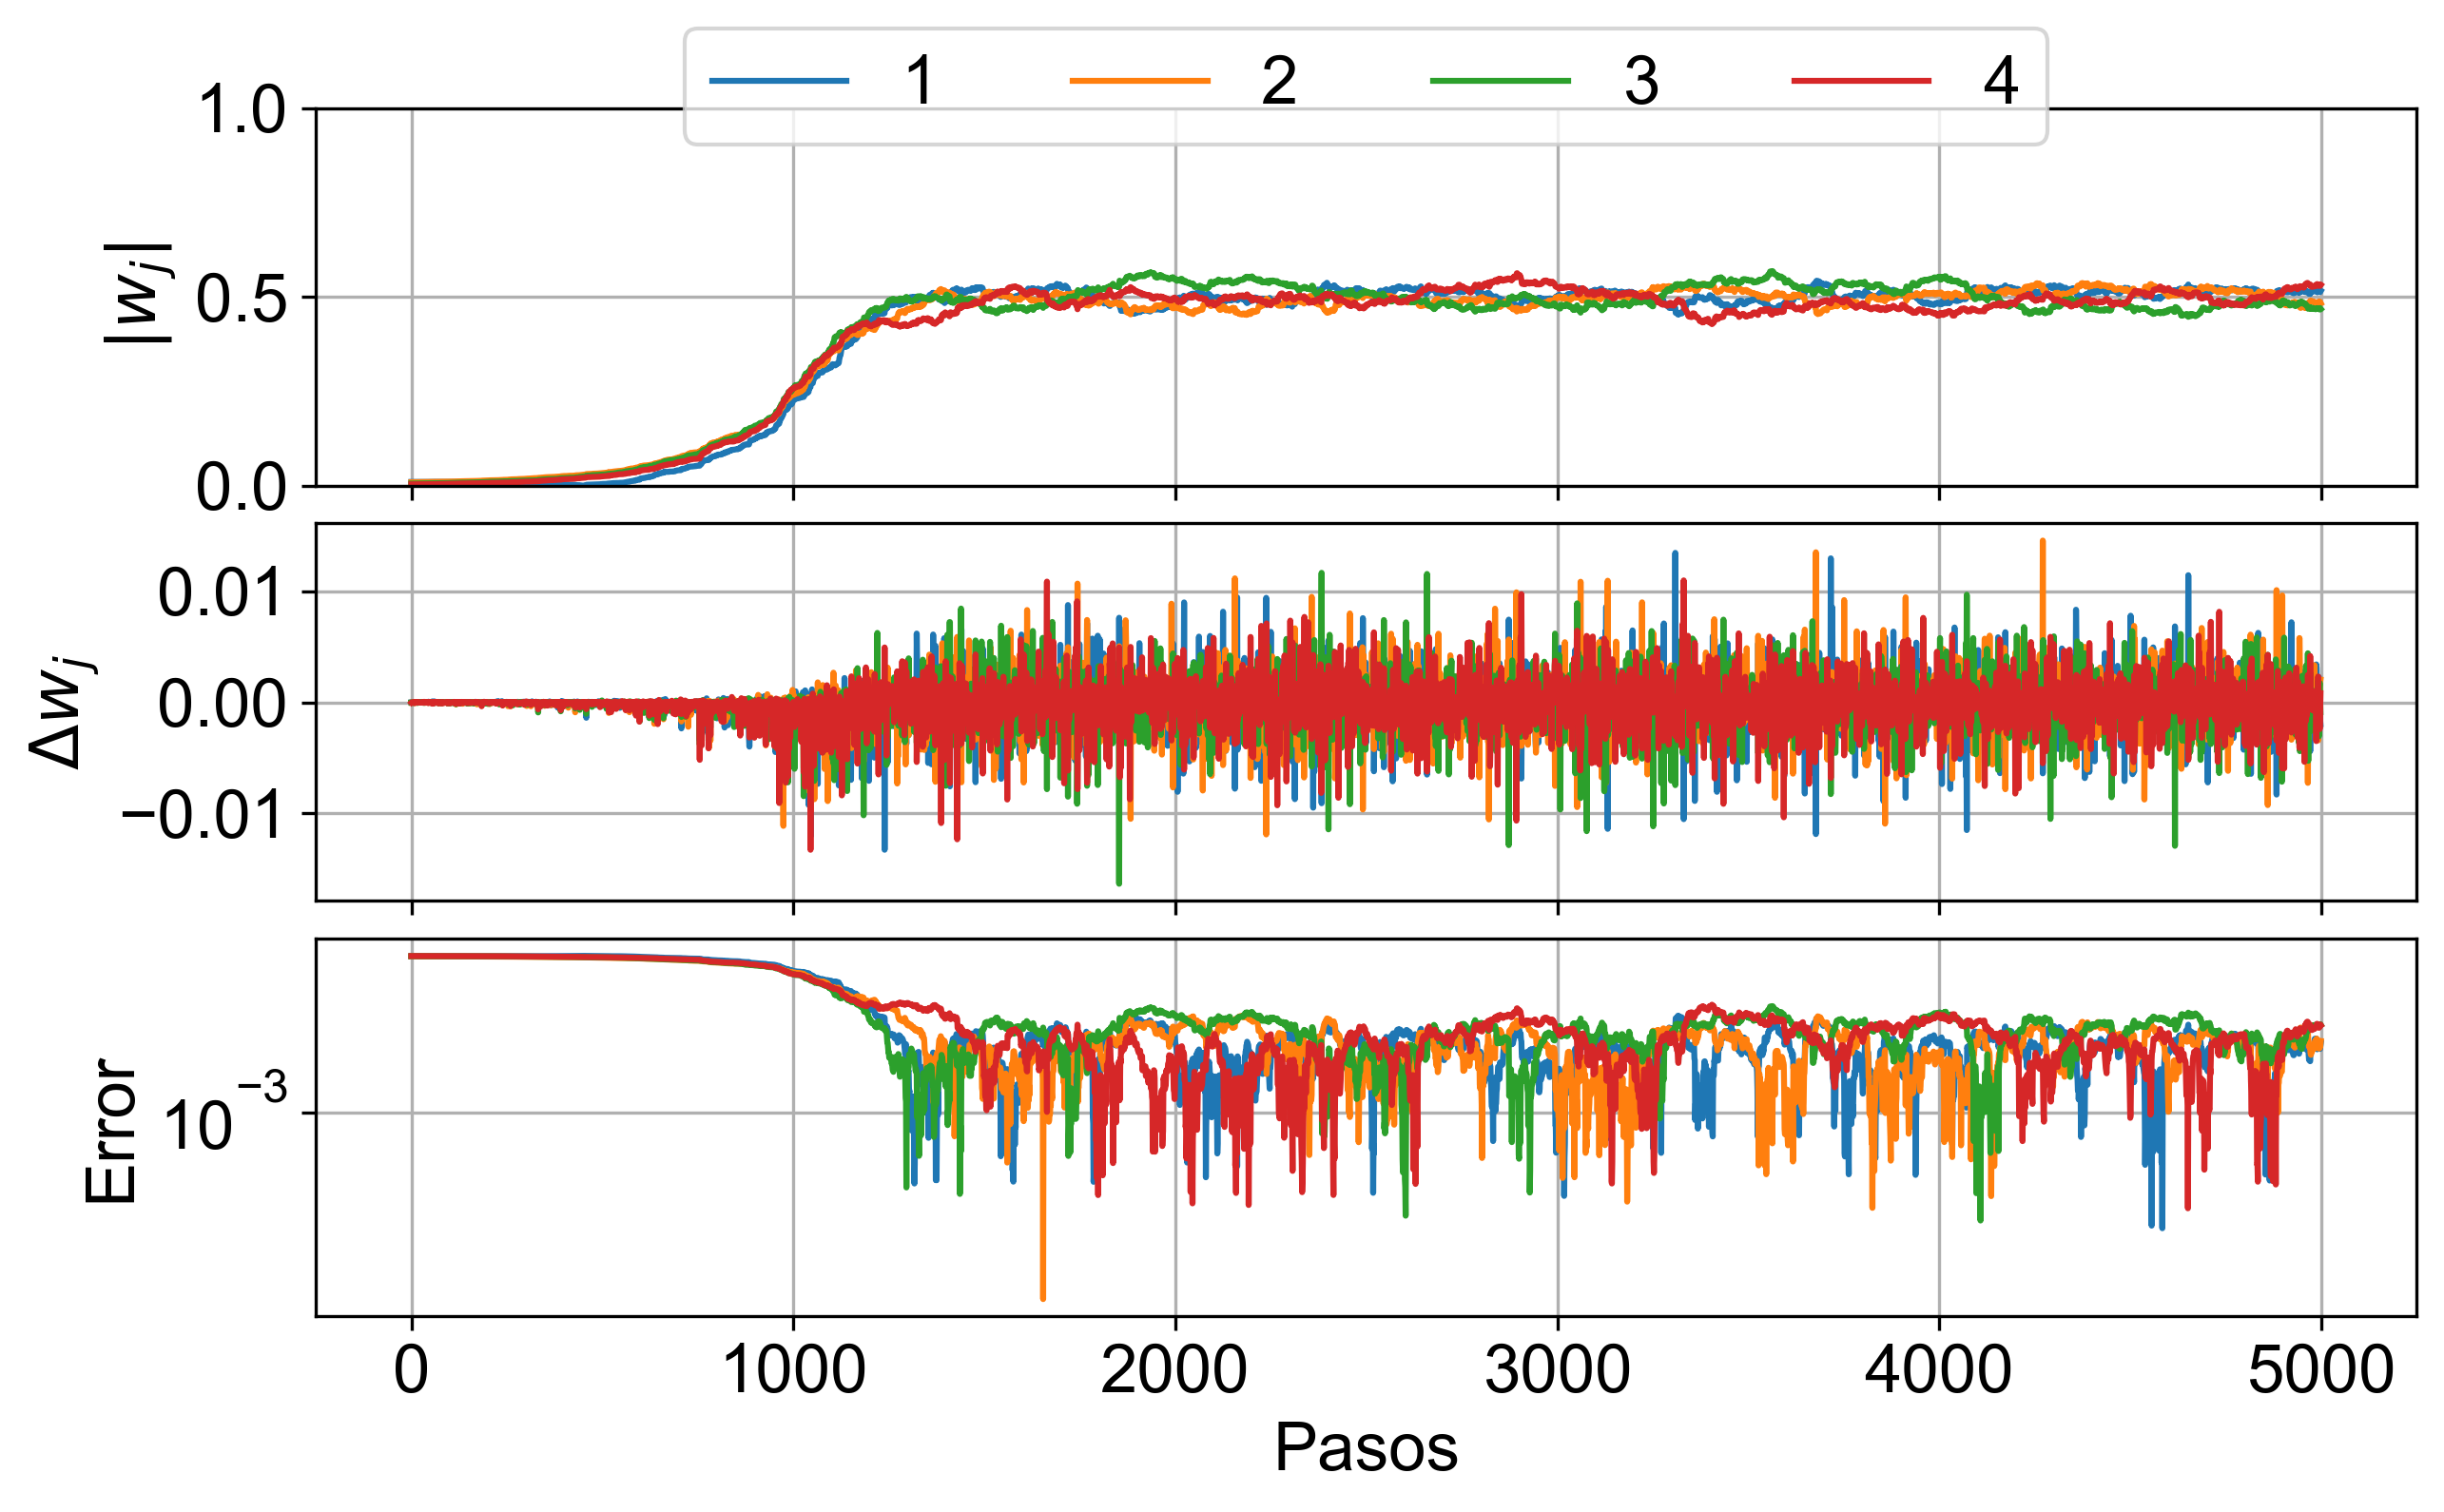
\includegraphics[width=\textwidth]{ej1_fig1.png}
      \caption{\label{fig:ej1_fig1}}
  \end{subfigure}
  \hfill
  \begin{subfigure}[b]{0.3\textwidth}
      \centering
      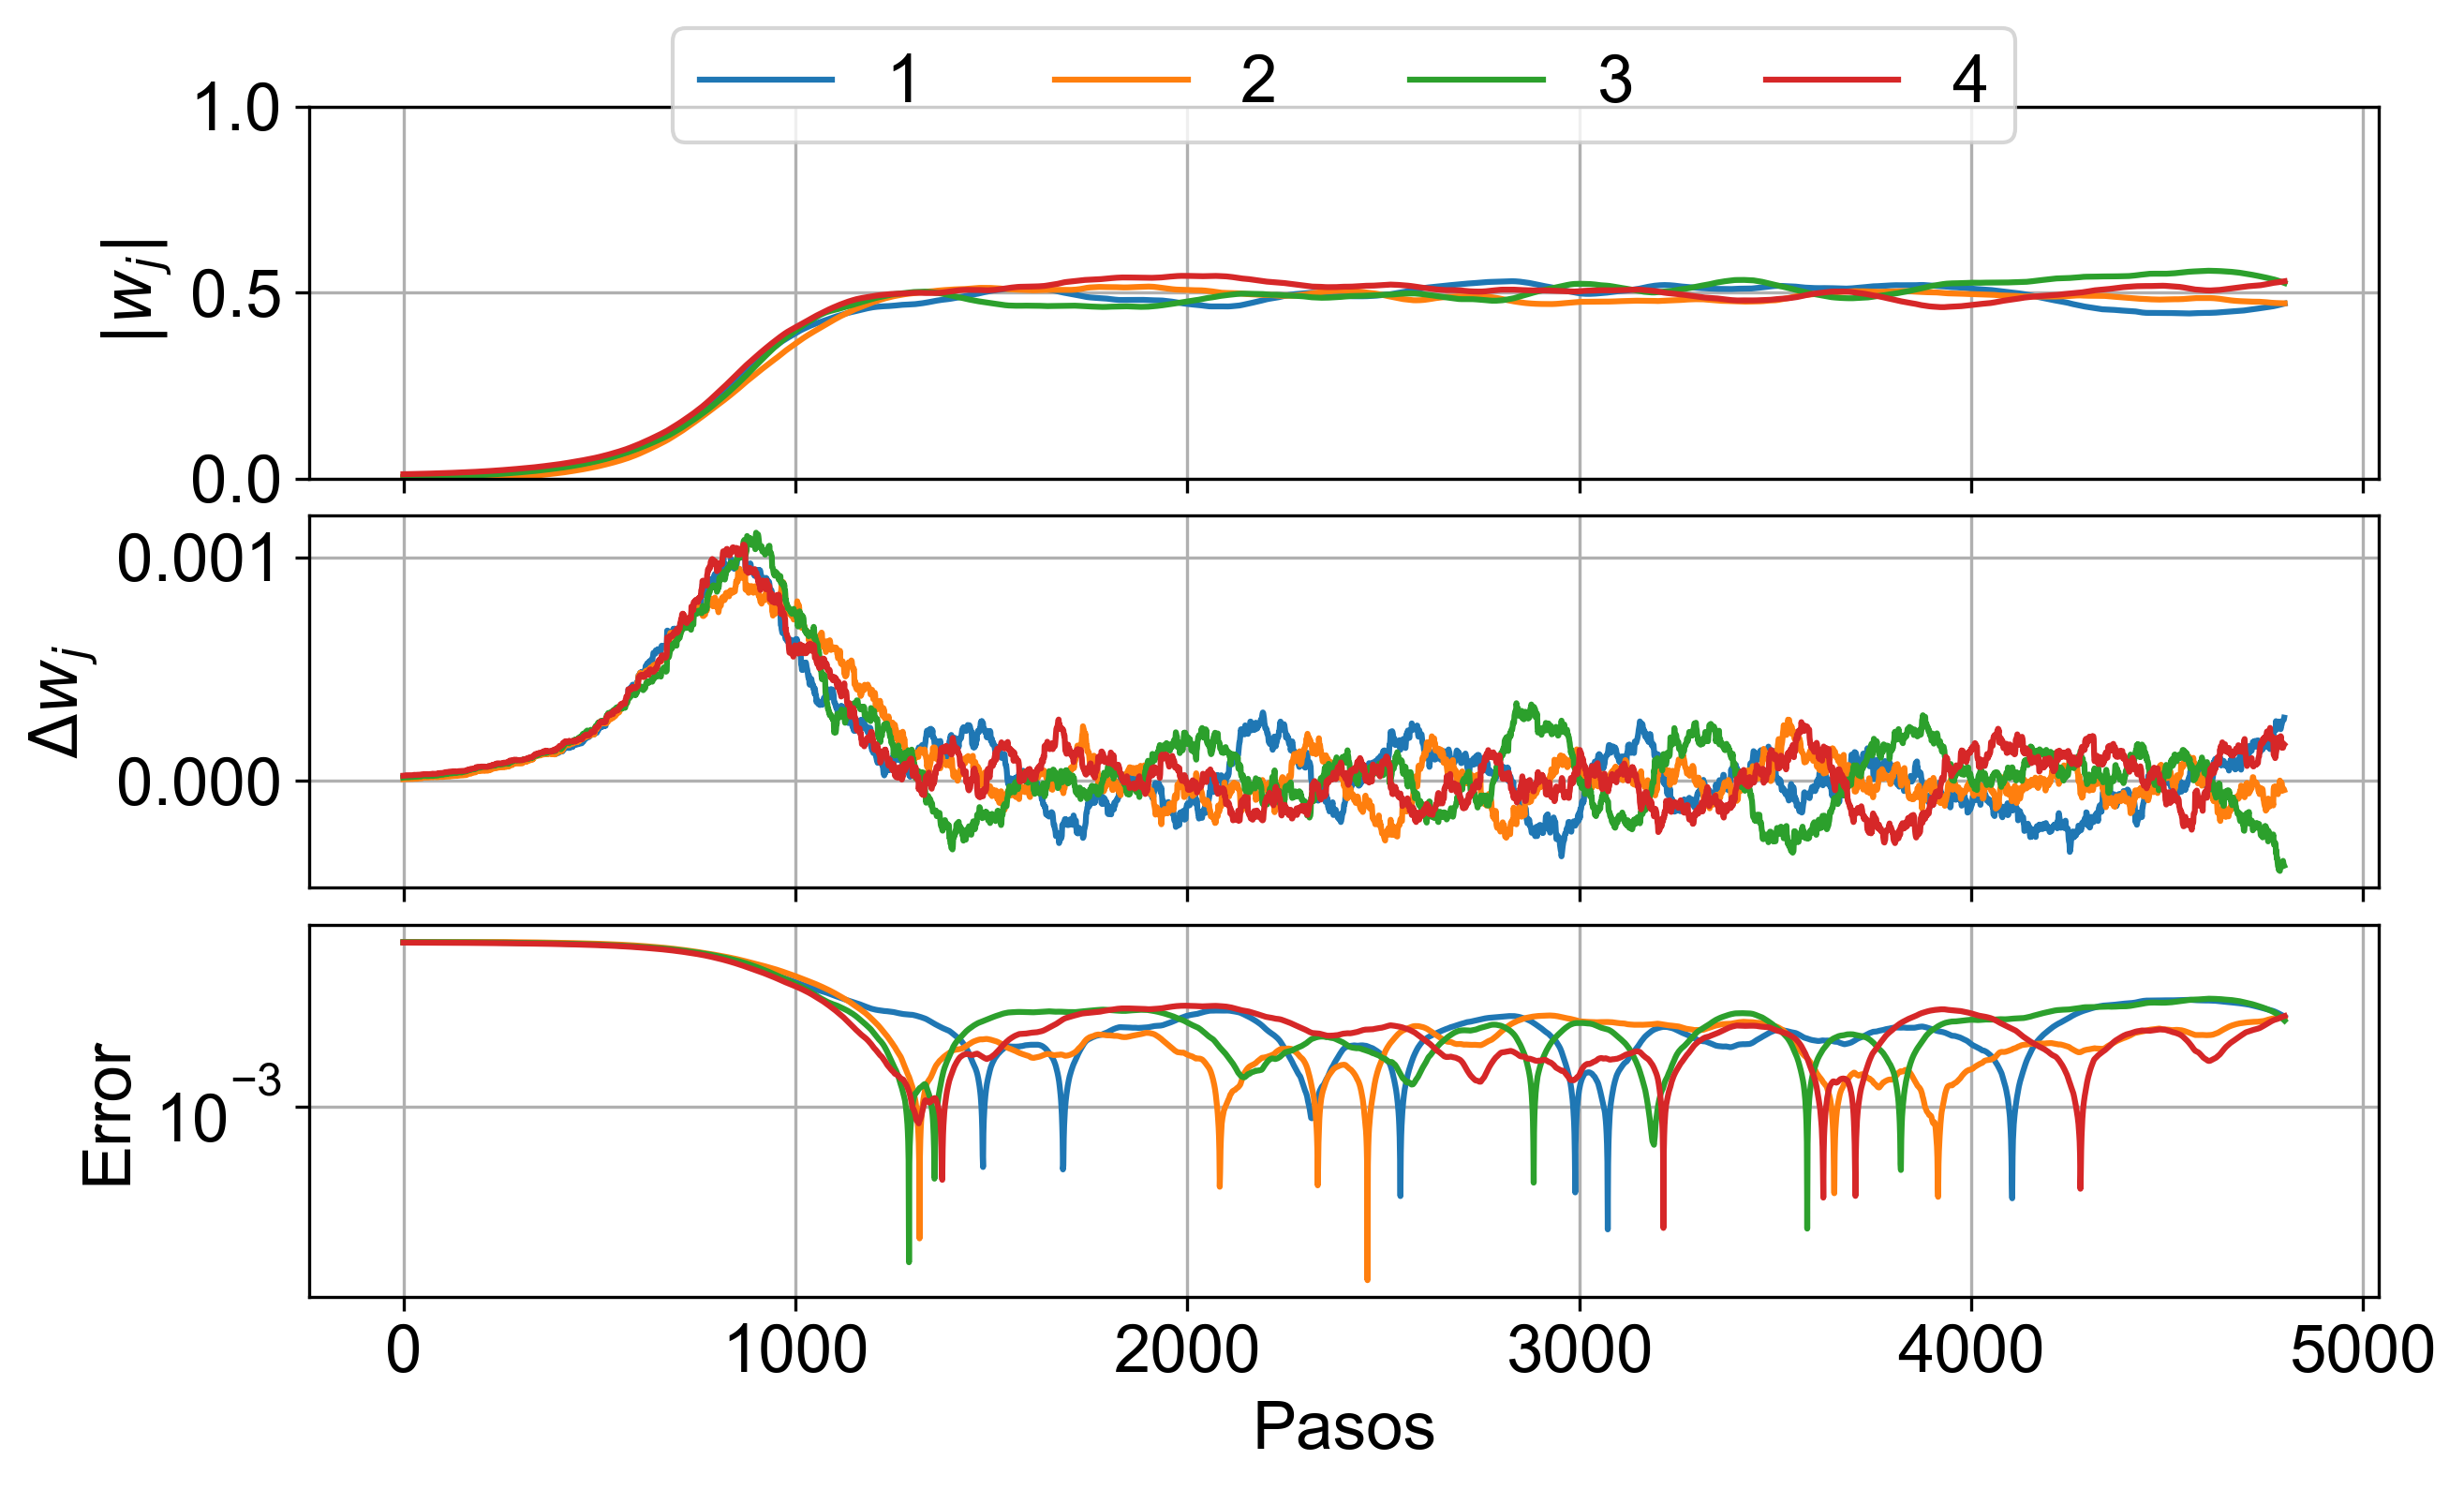
\includegraphics[width=\textwidth]{ej1_fig2.png}
      \caption{\label{fig:ej1_fig2}}
  \end{subfigure}
  \hfill
  \begin{subfigure}[b]{0.3\textwidth}
      \centering
      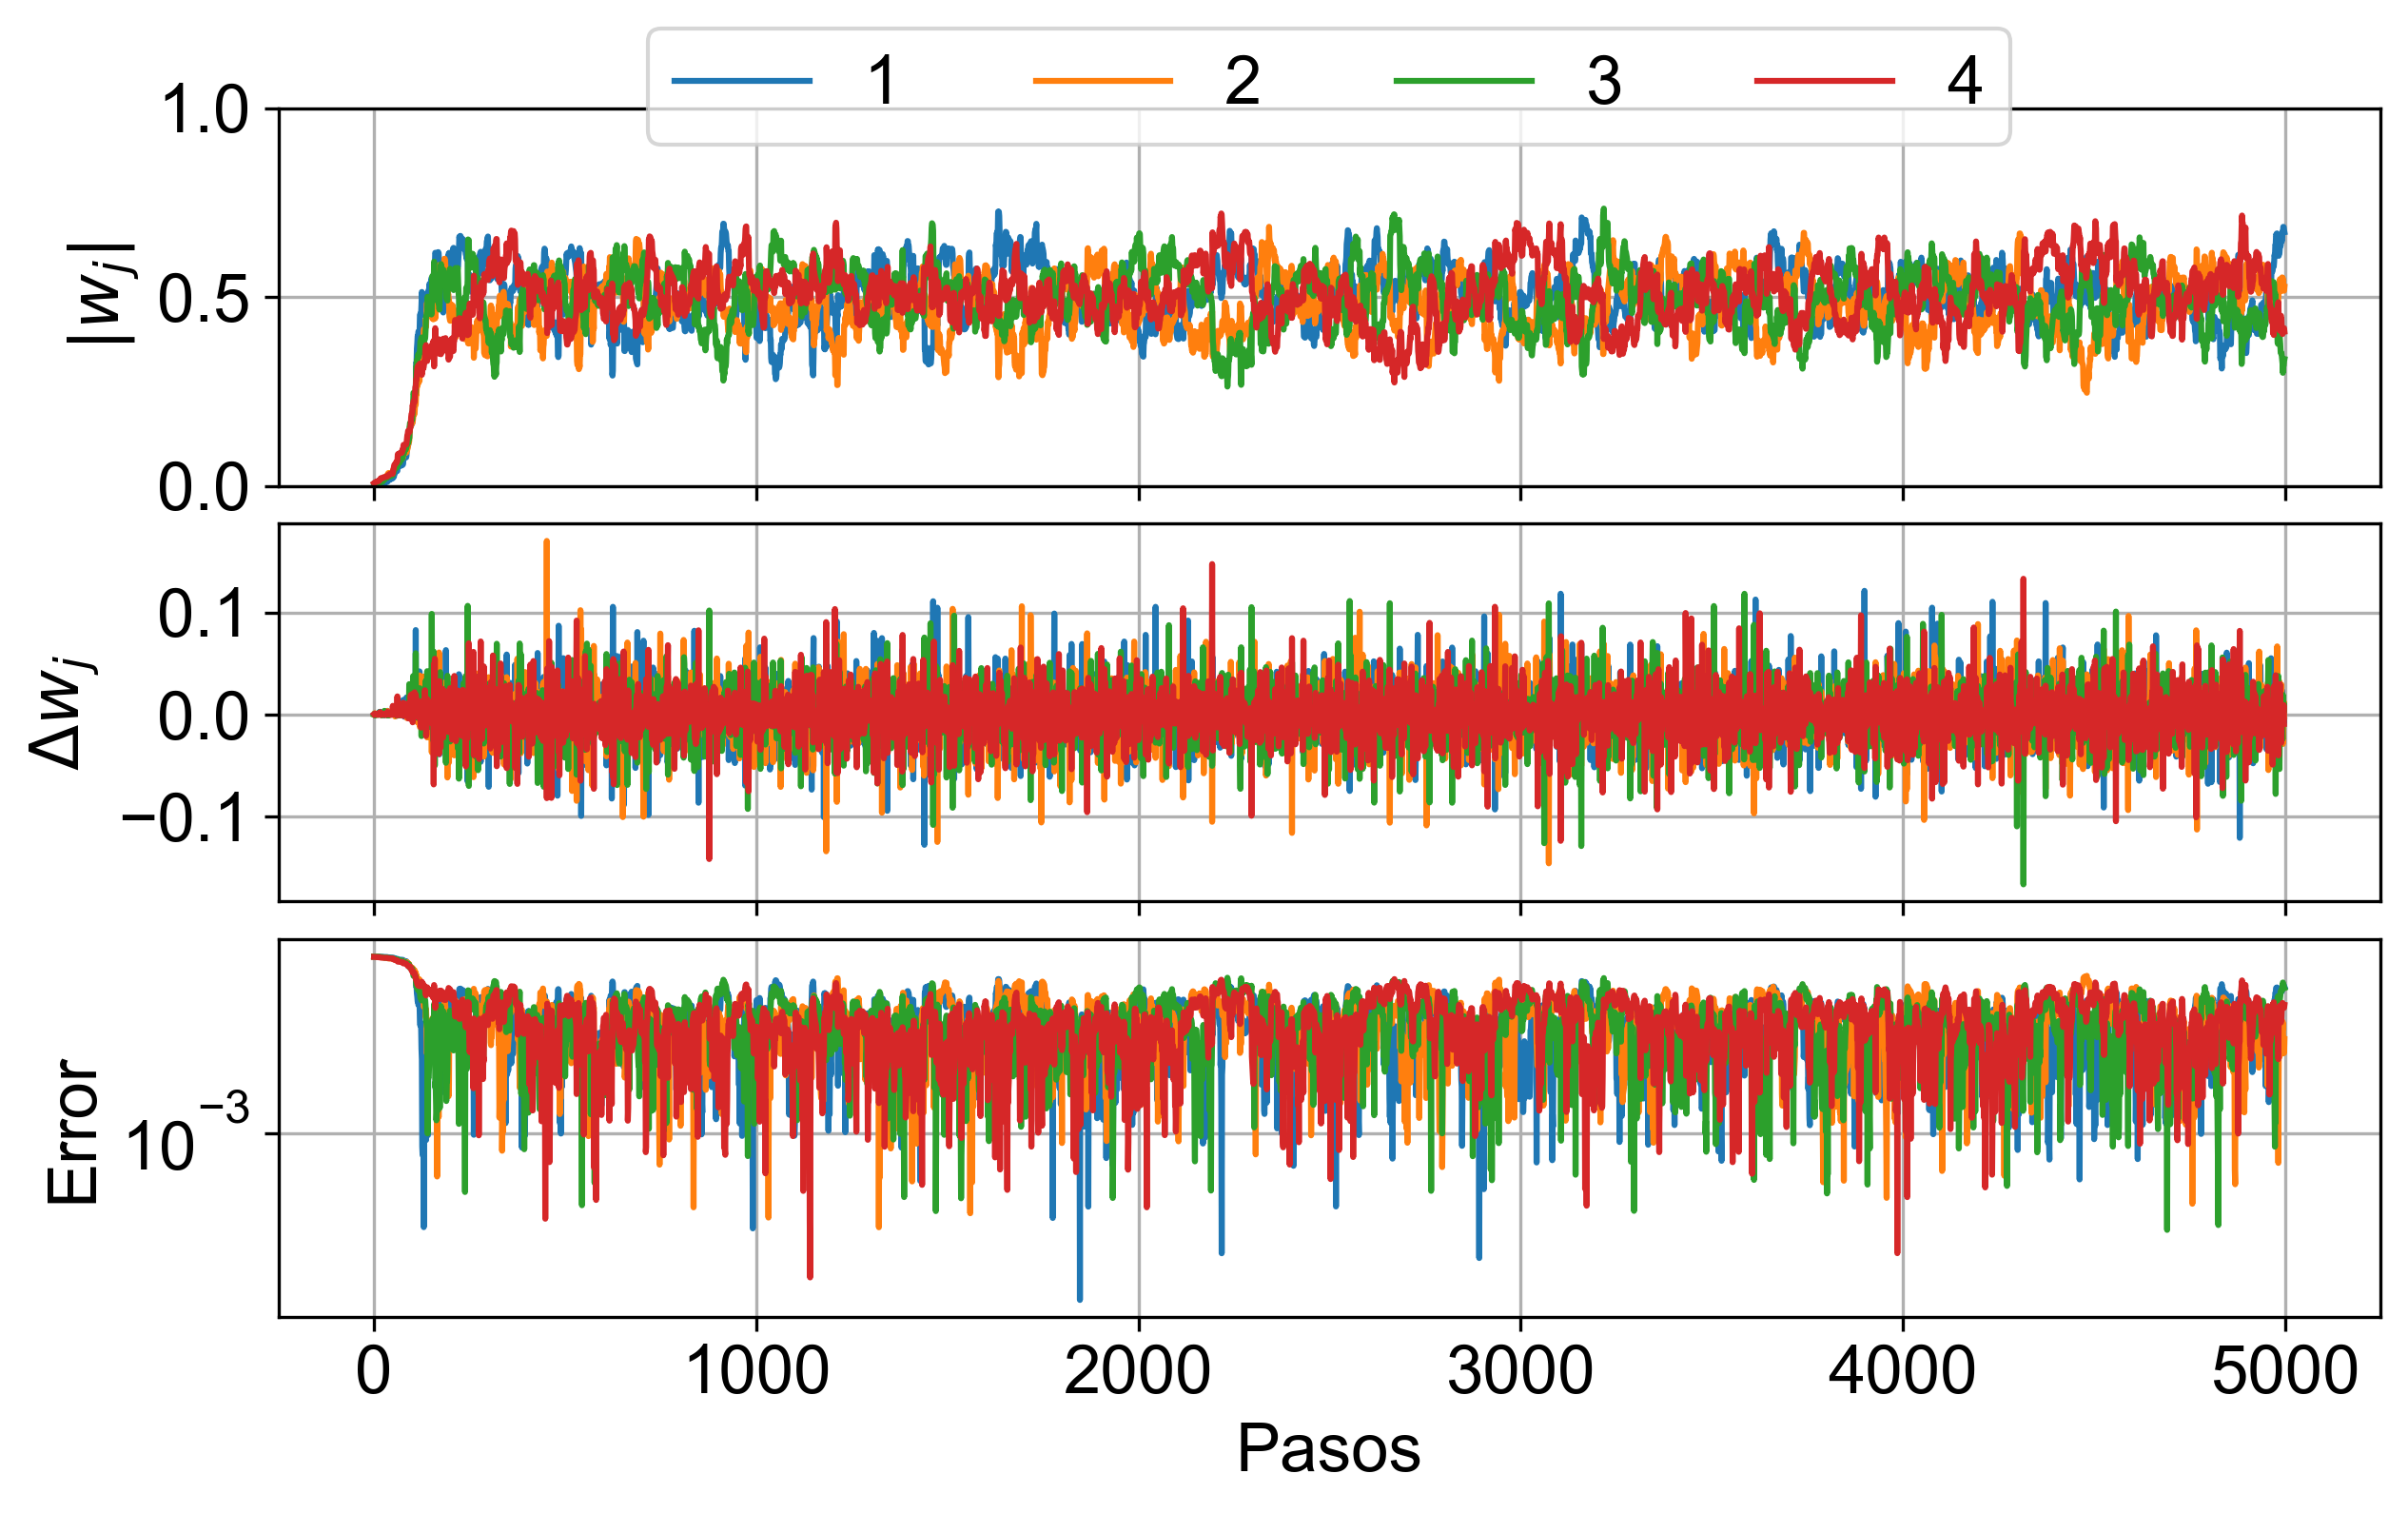
\includegraphics[width=\textwidth]{ej1_fig3.png}
      \caption{\label{fig:ej1_fig3}}
  \end{subfigure}
     \caption{Evolución del módulo de los pesos $w_j$, las modificaciones $\Delta w_j$ y la diferencia entre $w_j$ y $v_j$ durante el entrenamiento de la red neuronal. En \ref{sub@fig:ej1_fig1} se empleó una tasa de aprendizaje de $\eta = 0.001$. En \ref{sub@fig:ej1_fig2} se empleó la misma tasa de aprendizaje pero además se procesaron los datos promediando en cada paso de tiempo sobre los 200 pasos adyacentes. En \ref{sub@fig:ej1_fig3} se empleó una tasa de aprendizaje de $\eta = 0.01$.}
     \label{fig:three graphs}
\end{figure}

\begin{figure}
  \centering
  \begin{subfigure}[b]{0.24\textwidth}
      \centering
      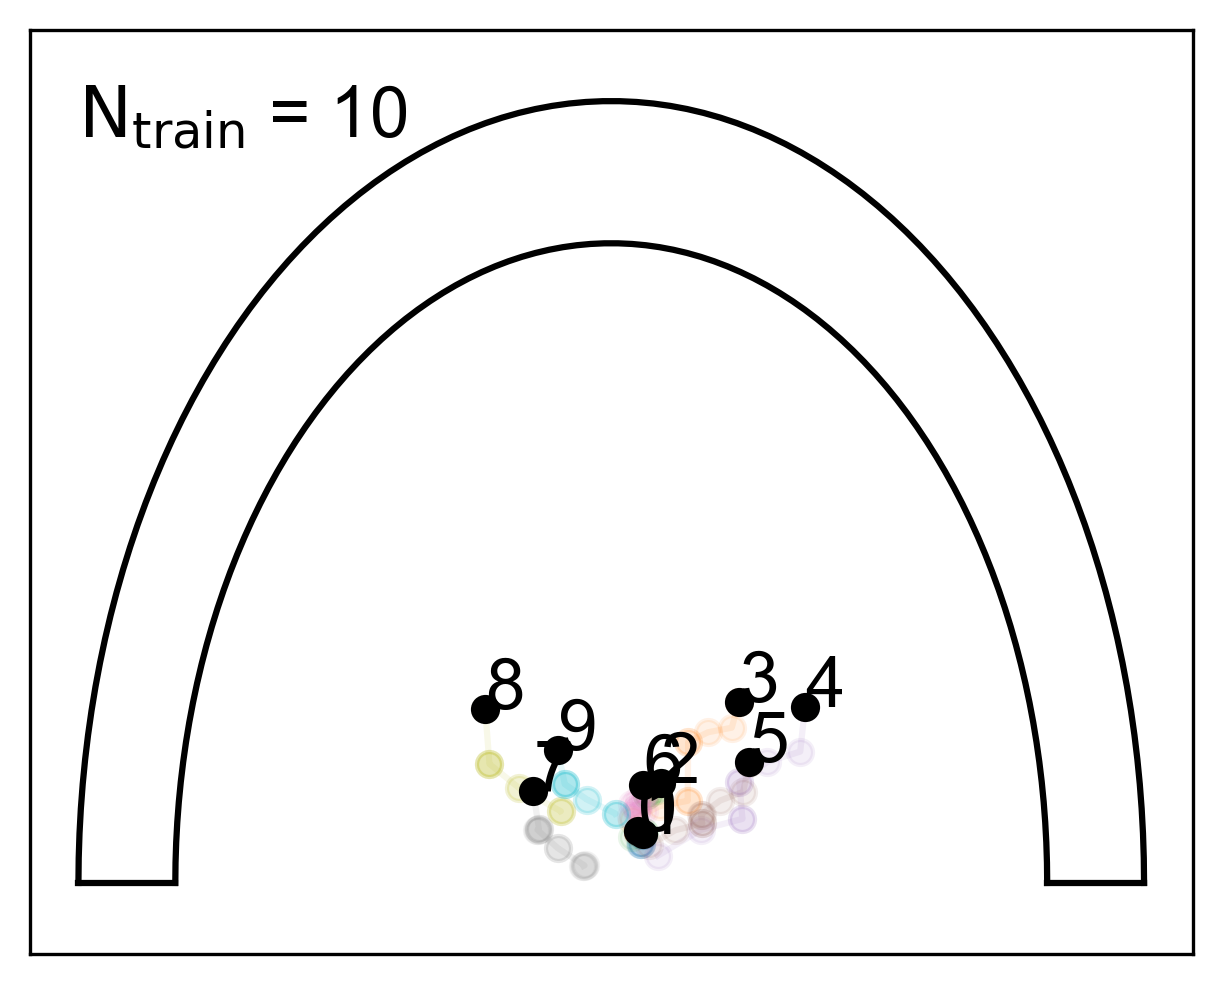
\includegraphics[width=\textwidth]{ej2_fig1_1.png}
      \caption{\label{fig:ej2_fig1_1}}
  \end{subfigure}
  \hfill
  \begin{subfigure}[b]{0.24\textwidth}
      \centering
      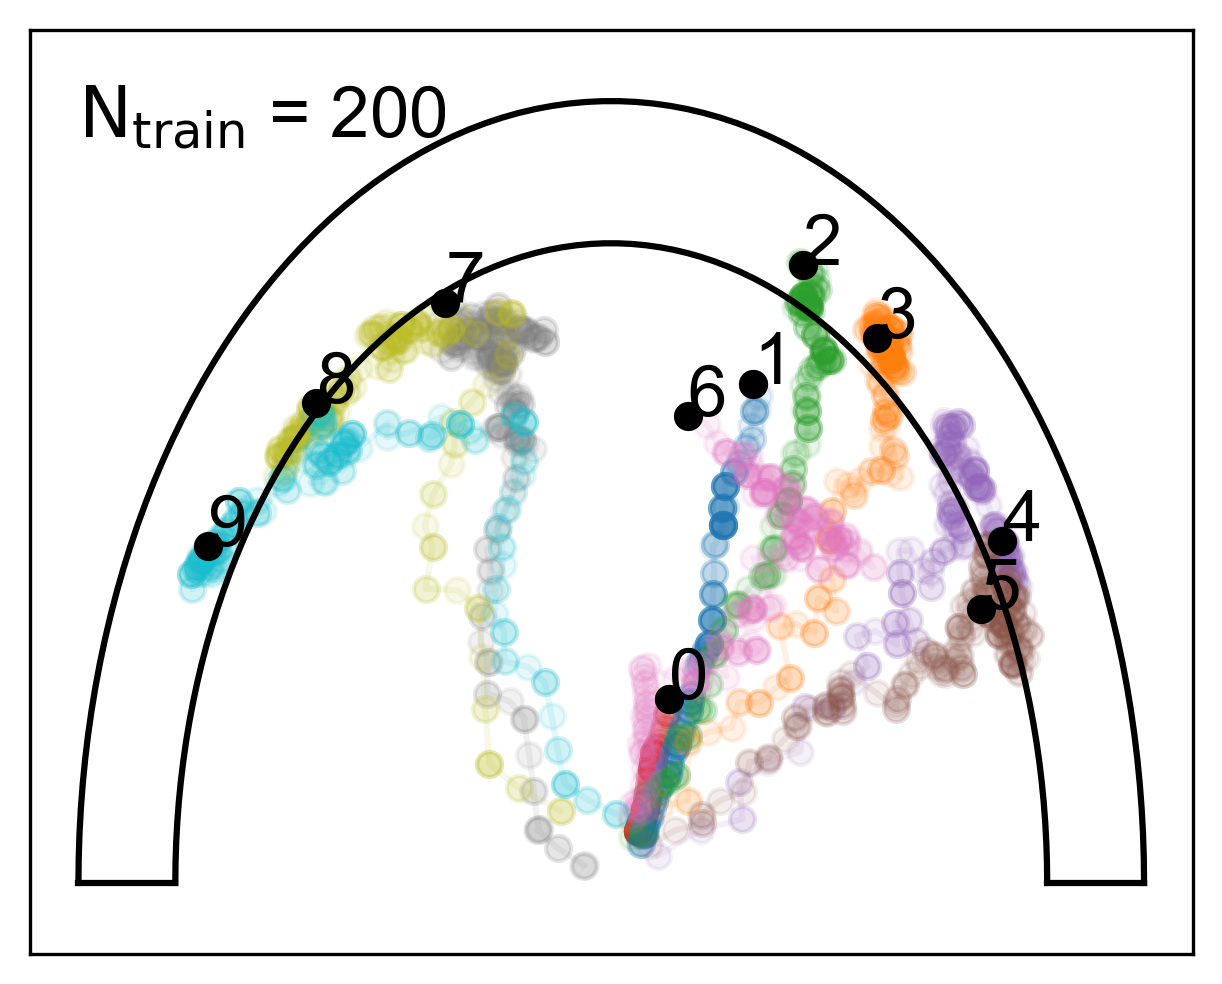
\includegraphics[width=\textwidth]{ej2_fig1_2.png}
      \caption{\label{fig:ej2_fig1_2}}
  \end{subfigure}
  \hfill
  \begin{subfigure}[b]{0.24\textwidth}
      \centering
      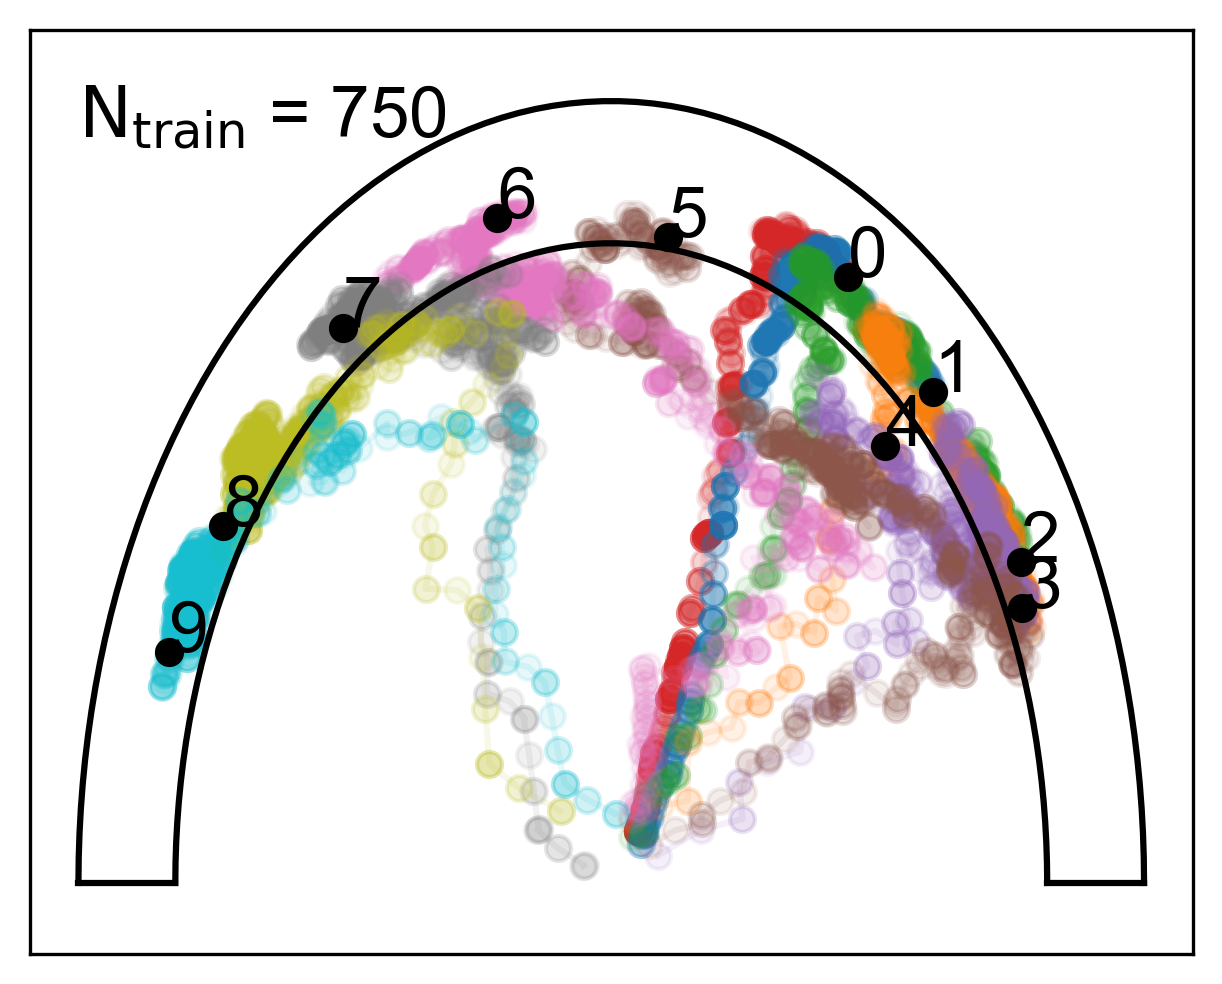
\includegraphics[width=\textwidth]{ej2_fig1_3.png}
      \caption{\label{fig:ej2_fig1_3}}
  \end{subfigure}
  \hfill
  \begin{subfigure}[b]{0.24\textwidth}
      \centering
      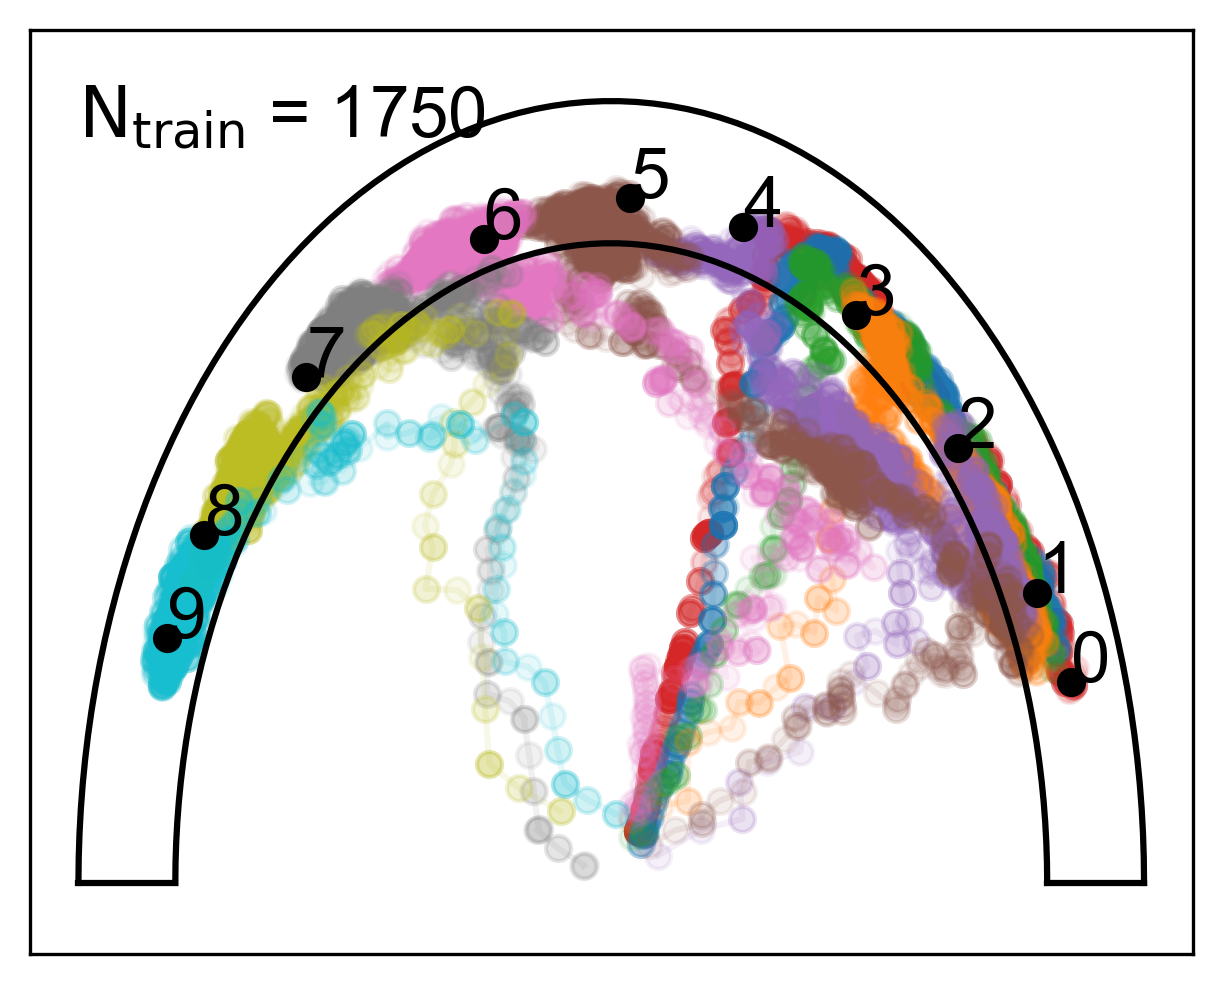
\includegraphics[width=\textwidth]{ej2_fig1_4.png}
      \caption{\label{fig:ej2_fig1_4}}
  \end{subfigure}
     \caption{$\sigma = 1$, $\eta = 0.1$}
     \label{fig:ej2_fig1}
\end{figure}

\begin{figure}
  \centering
  \begin{subfigure}[b]{0.24\textwidth}
      \centering
      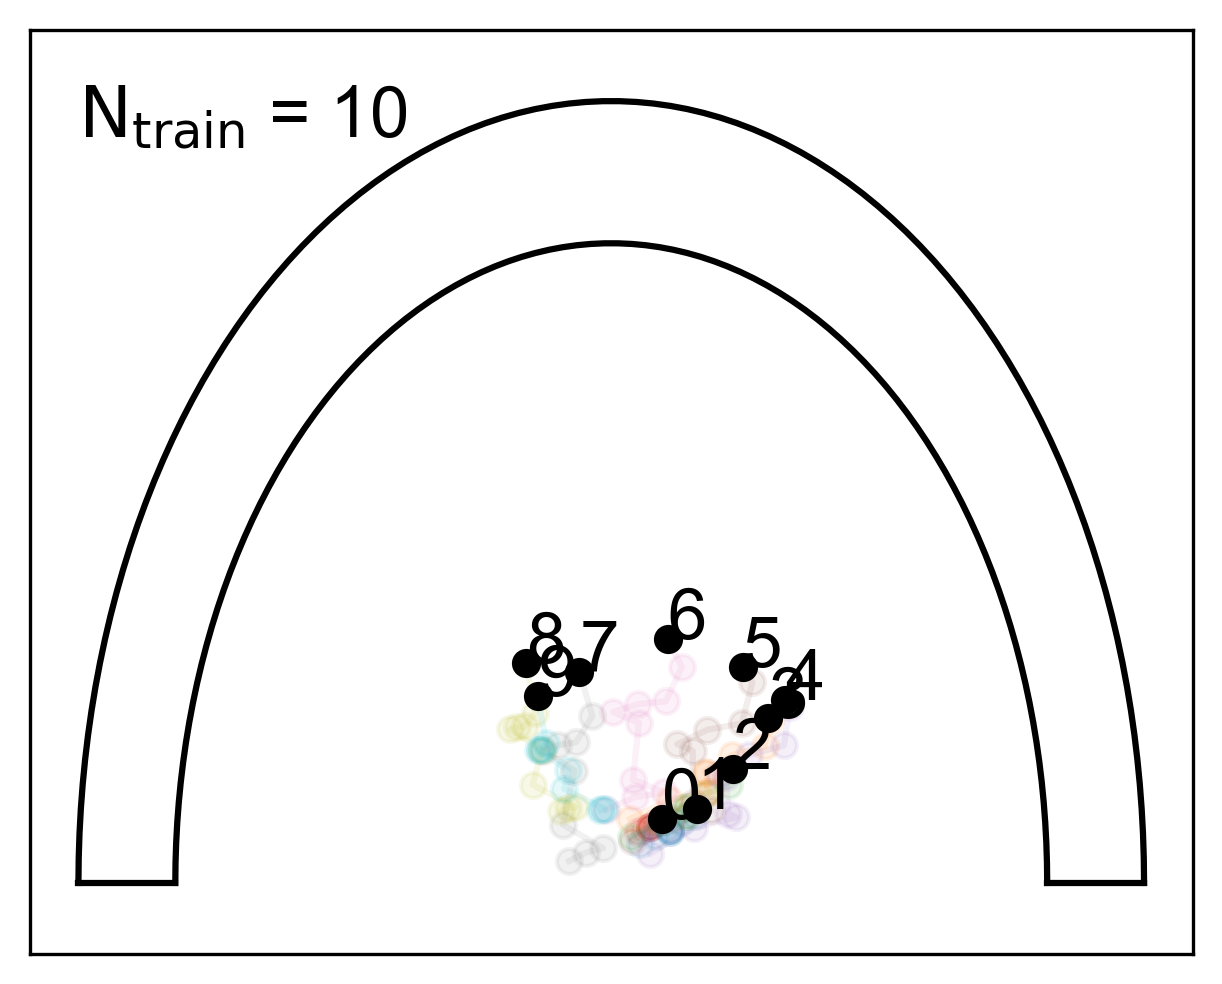
\includegraphics[width=\textwidth]{ej2_fig2_1.png}
      \caption{\label{fig:ej2_fig2_1}}
  \end{subfigure}
  \hfill
  \begin{subfigure}[b]{0.24\textwidth}
      \centering
      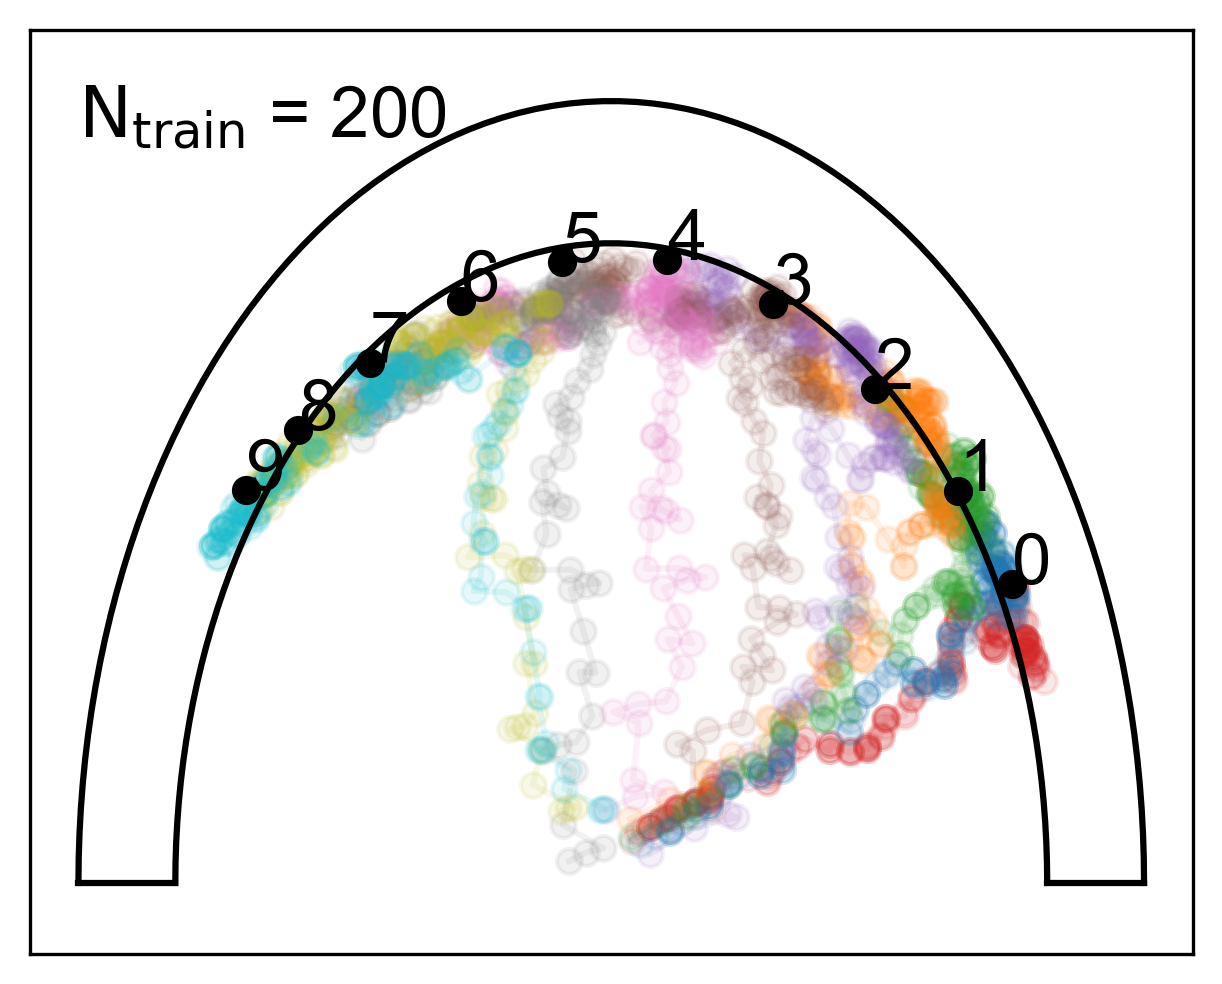
\includegraphics[width=\textwidth]{ej2_fig2_2.png}
      \caption{\label{fig:ej2_fig2_2}}
  \end{subfigure}
  \hfill
  \begin{subfigure}[b]{0.24\textwidth}
      \centering
      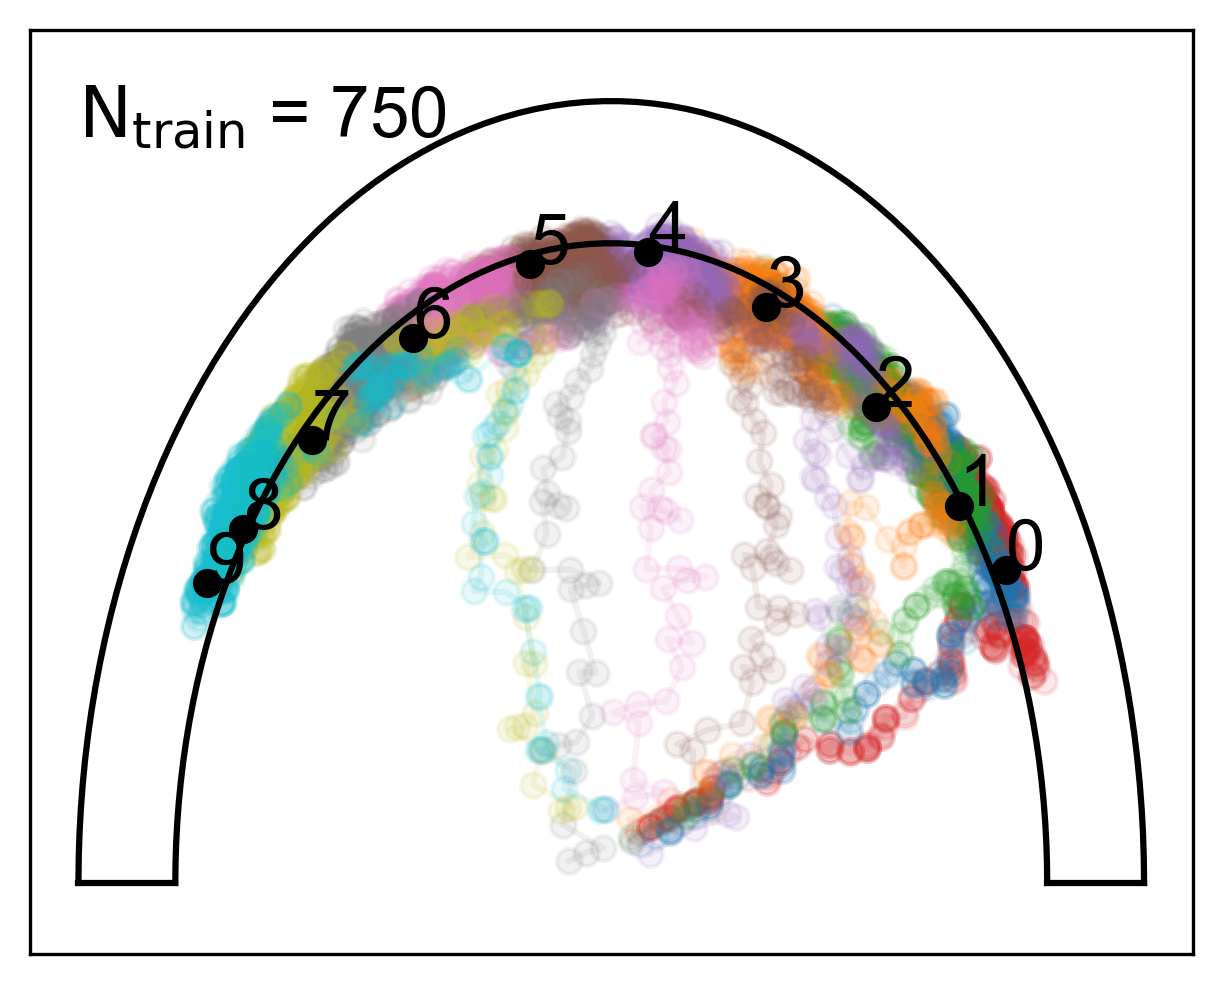
\includegraphics[width=\textwidth]{ej2_fig2_3.png}
      \caption{\label{fig:ej2_fig2_3}}
  \end{subfigure}
  \hfill
  \begin{subfigure}[b]{0.24\textwidth}
      \centering
      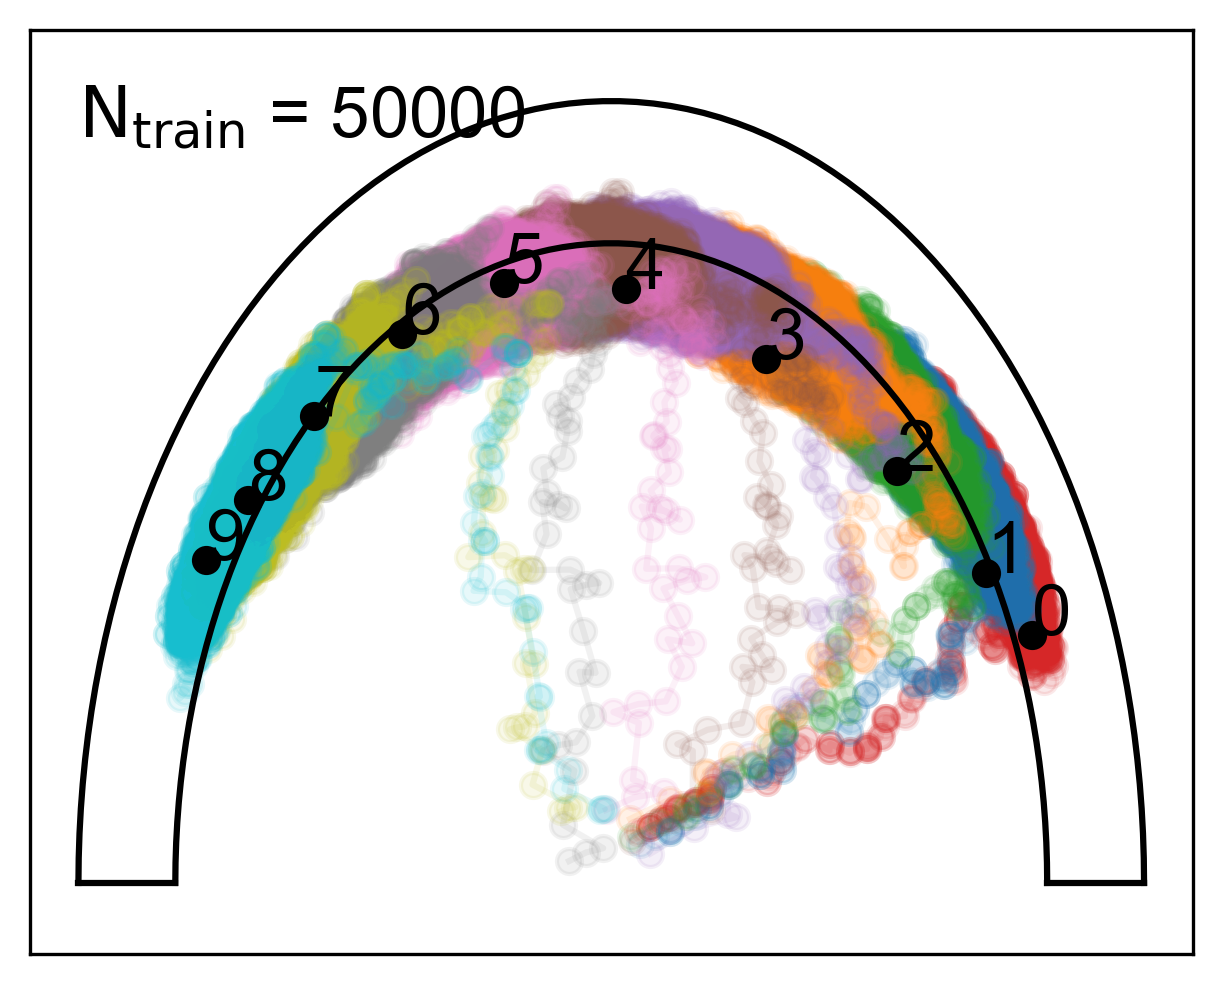
\includegraphics[width=\textwidth]{ej2_fig2_4.png}
      \caption{\label{fig:ej2_fig2_4}}
  \end{subfigure}
     \caption{$\sigma = 2$, $\eta = 0.1$}
     \label{fig:ej2_fig2}
\end{figure}


\begin{figure}
  \centering
  \begin{subfigure}[b]{0.24\textwidth}
      \centering
      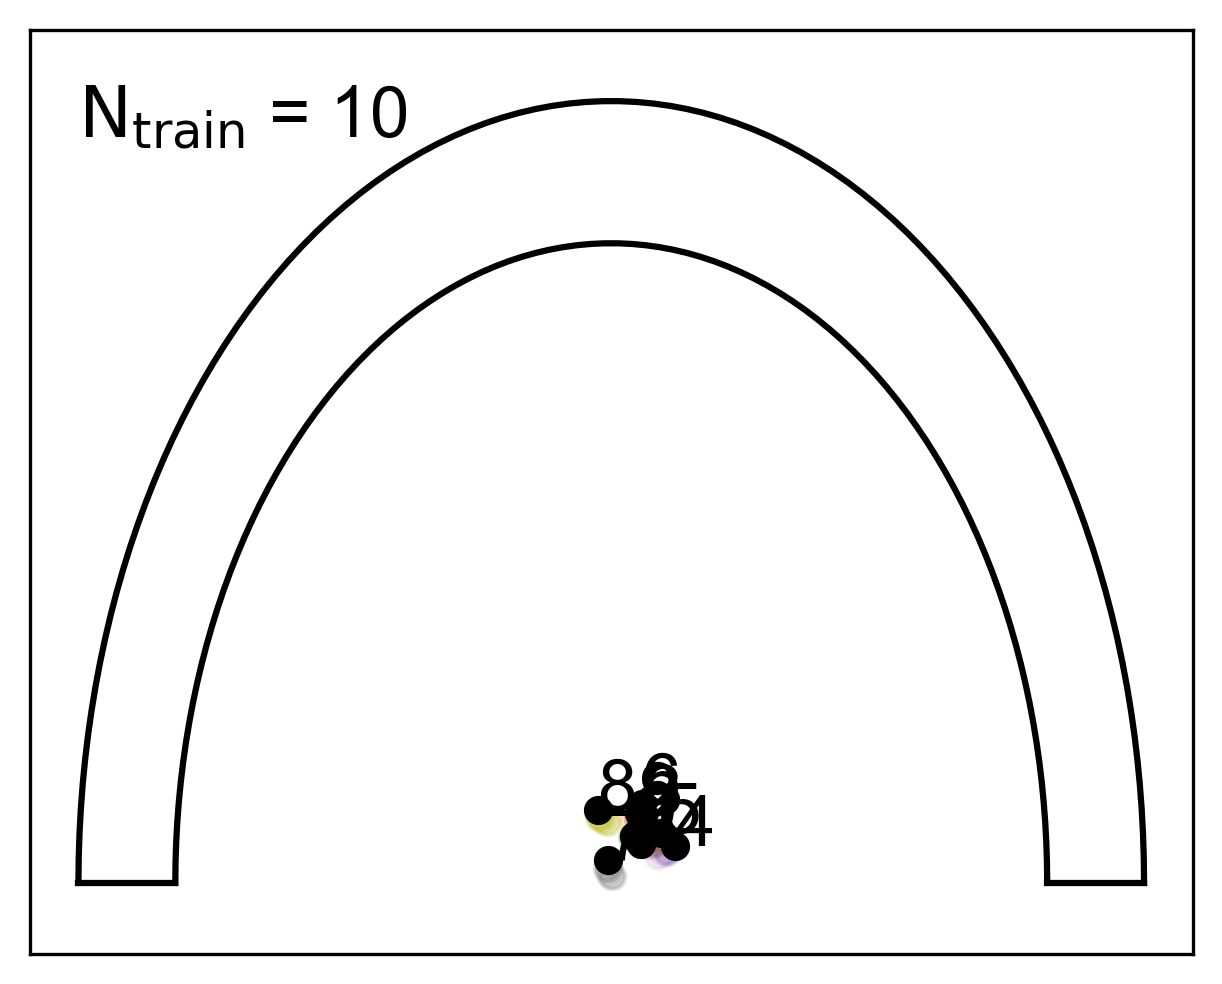
\includegraphics[width=\textwidth]{ej2_fig3_1.png}
      \caption{\label{fig:ej2_fig3_1}}
  \end{subfigure}
  \hfill
  \begin{subfigure}[b]{0.24\textwidth}
      \centering
      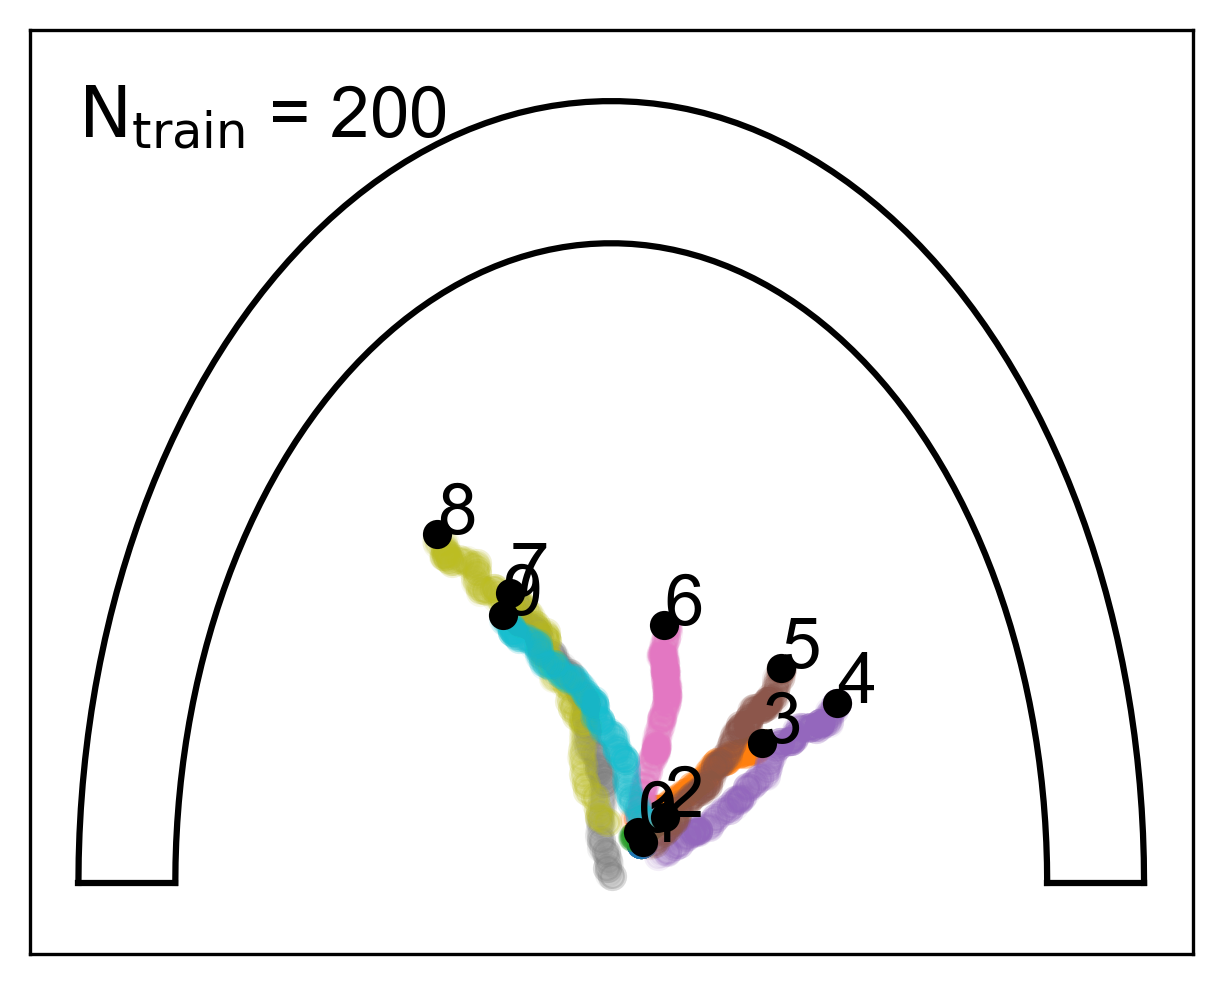
\includegraphics[width=\textwidth]{ej2_fig3_2.png}
      \caption{\label{fig:ej2_fig3_2}}
  \end{subfigure}
  \hfill
  \begin{subfigure}[b]{0.24\textwidth}
      \centering
      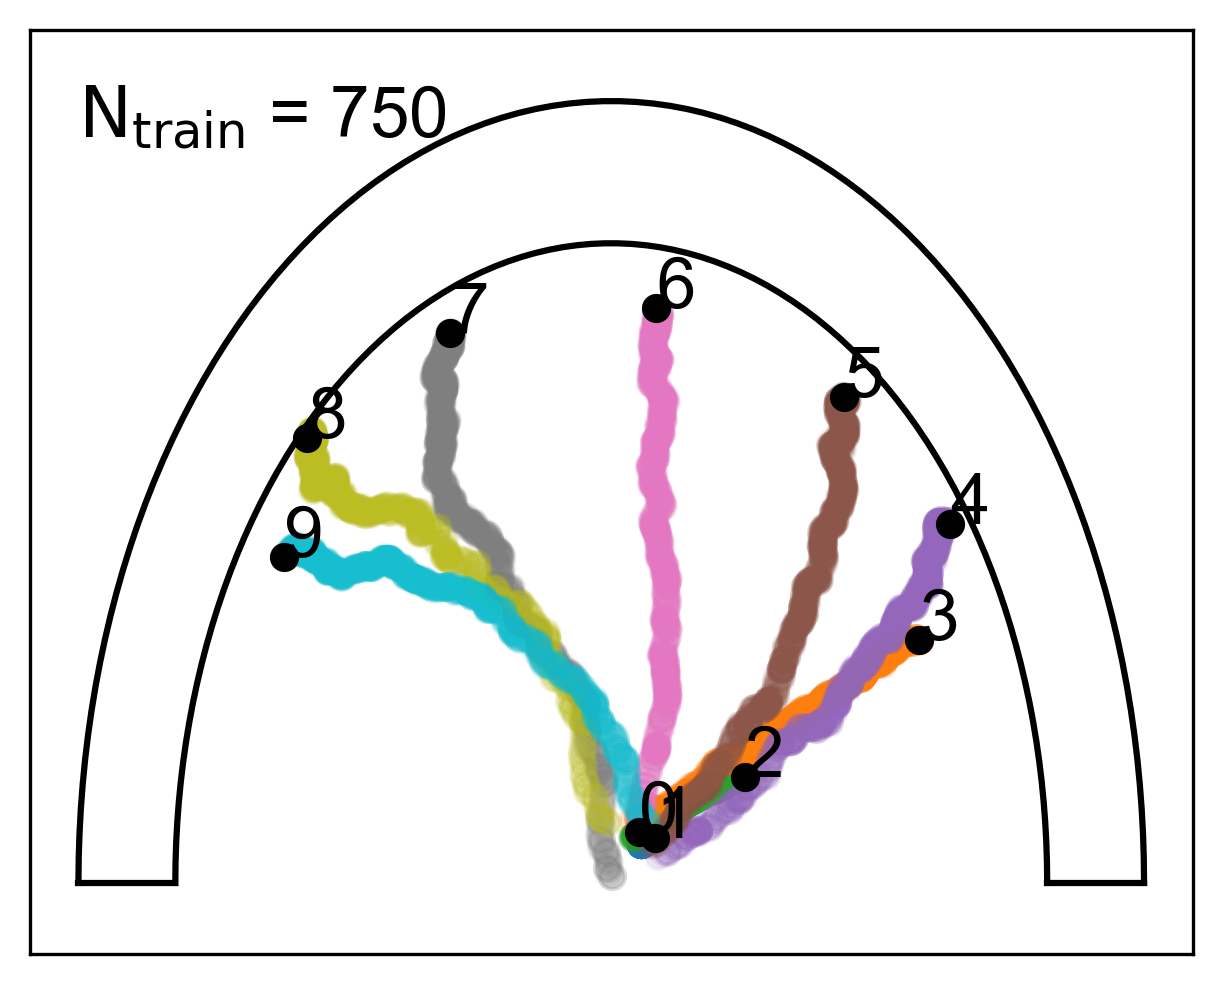
\includegraphics[width=\textwidth]{ej2_fig3_3.png}
      \caption{\label{fig:ej2_fig3_3}}
  \end{subfigure}
  \hfill
  \begin{subfigure}[b]{0.24\textwidth}
      \centering
      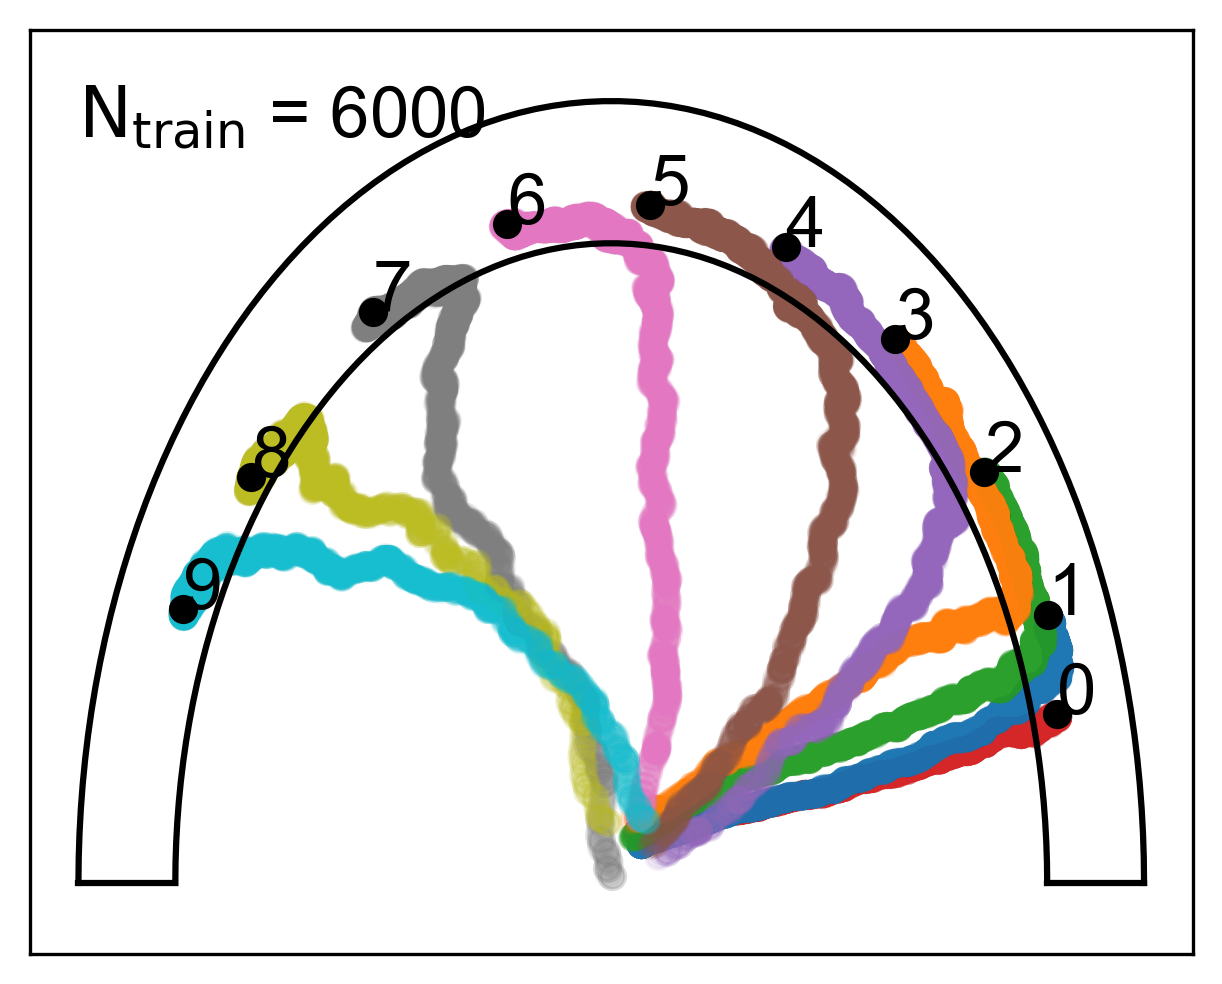
\includegraphics[width=\textwidth]{ej2_fig3_4.png}
      \caption{\label{fig:ej2_fig3_4}}
  \end{subfigure}
     \caption{$\sigma = 1$, $\eta = 0.01$}
     \label{fig:ej2_fig3}
\end{figure}



\section*{Apéndice}
A continuación se desarrolla el código empleado durante este trabajo implementado en Python.




\begin{lstlisting}[language=Python]
  #Import libraries
  import numpy as np
  import matplotlib
  import matplotlib.pyplot as plt
  import tensorflow as tf
  
  

\end{lstlisting}

\bibliography{Chehade_practica_5.bib}

\end{document}





